% When Fusion Breaks — paper skeleton.
% Figures are generated by `make figures` and never edited by hand, so a figure can
% never disagree with the results JSON it summarises.
\documentclass[11pt,a4paper]{article}

\usepackage[utf8]{inputenc}
\usepackage[T1]{fontenc}
\usepackage{microtype}
\usepackage{graphicx}
\usepackage{booktabs}
\usepackage{amsmath}
\usepackage{amssymb}
\usepackage[hidelinks]{hyperref}
\usepackage[margin=1in]{geometry}
\usepackage{natbib}
\usepackage{caption}

\title{When Fusion Breaks:\\
       Graceful Degradation in Multimodal Emotion Recognition}
\author{Inayat}
\date{\today}

\begin{document}
\maketitle

\begin{abstract}
Multimodal models fuse text, audio and video and outperform unimodal models on
benchmarks. Benchmark evaluation, however, assumes every modality is present and clean —
an assumption deployments violate routinely. We evaluate \textbf{N} fusion architectures
across \textbf{M} corruption regimes on two datasets and show that
\textbf{[architecture class]} retains \textbf{X\%} of clean performance at \textbf{Y}
corruption while \textbf{[other class]} retains \textbf{Z\%}.
% ^ This sentence is the paper. Fill in the letters from experiments/results/REPORT.md.
\end{abstract}

\section{Introduction}
% The gap: benchmark numbers are computed under conditions deployments never see.
% H1, stated before the experiments, and falsifiable either way.

\section{Related work}
% Fusion architectures: TFN, LMF, MulT, MISA, Self-MM.
% Missing-modality work: mostly binary absence, mostly one architecture at a time.
% Robustness benchmarks in vision/NLP (ImageNet-C and descendants) — the methodological
% template we are importing into multimodal affect.

\section{Method}
\subsection{Architectures}
% Six points on a fusion-sophistication axis, with encoder family, capacity and optimiser
% held fixed so the axis is the only thing that varies.

\subsection{Corruption protocol}
% Normalised severity; exact identity at severity 0; per-sample derived seeds so every
% architecture sees bit-identical corrupted inputs.

\subsection{Degradation metrics}
Retention is measured as skill above chance rather than as a raw ratio:
\begin{equation}
  \mathrm{Retention}(c) = \frac{m(c) - m_{\text{chance}}}{m(\text{clean}) - m_{\text{chance}}}
\end{equation}
% Justify: binary accuracy floors at 0.5, so an uncorrected ratio compresses every
% reliance score into the top third of its range and distorts comparisons between models
% with different clean scores.
\begin{equation}
  \mathrm{AUDC} = \frac{1}{s_{\max} - s_{\min}} \int_{s_{\min}}^{s_{\max}}
                  \mathrm{Retention}(s)\, \mathrm{d}s
\end{equation}
\begin{equation}
  \mathrm{MRS}(m) = 1 - \mathrm{Retention}(\text{remove } m)
\end{equation}

\section{Experimental setup}
% Datasets, splits (frozen and committed), 5 seeds, paired bootstrap with
% Holm--Bonferroni correction.

\subsection{Reproduction gate}
% No degradation claim precedes this table. See docs/REPRODUCTION.md.
\begin{table}[t]
  \centering
  \caption{Clean-data reproduction against published results.}
  \begin{tabular}{llrrr}
    \toprule
    Model & Dataset & Published & Ours & $\Delta$ \\
    \midrule
    MulT & MOSI & --- & --- & --- \\
    LMF  & MOSI & --- & --- & --- \\
    \bottomrule
  \end{tabular}
\end{table}

\section{Results}

\subsection{H1: does sophistication predict brittleness?}
\begin{figure}[t]
  \centering
  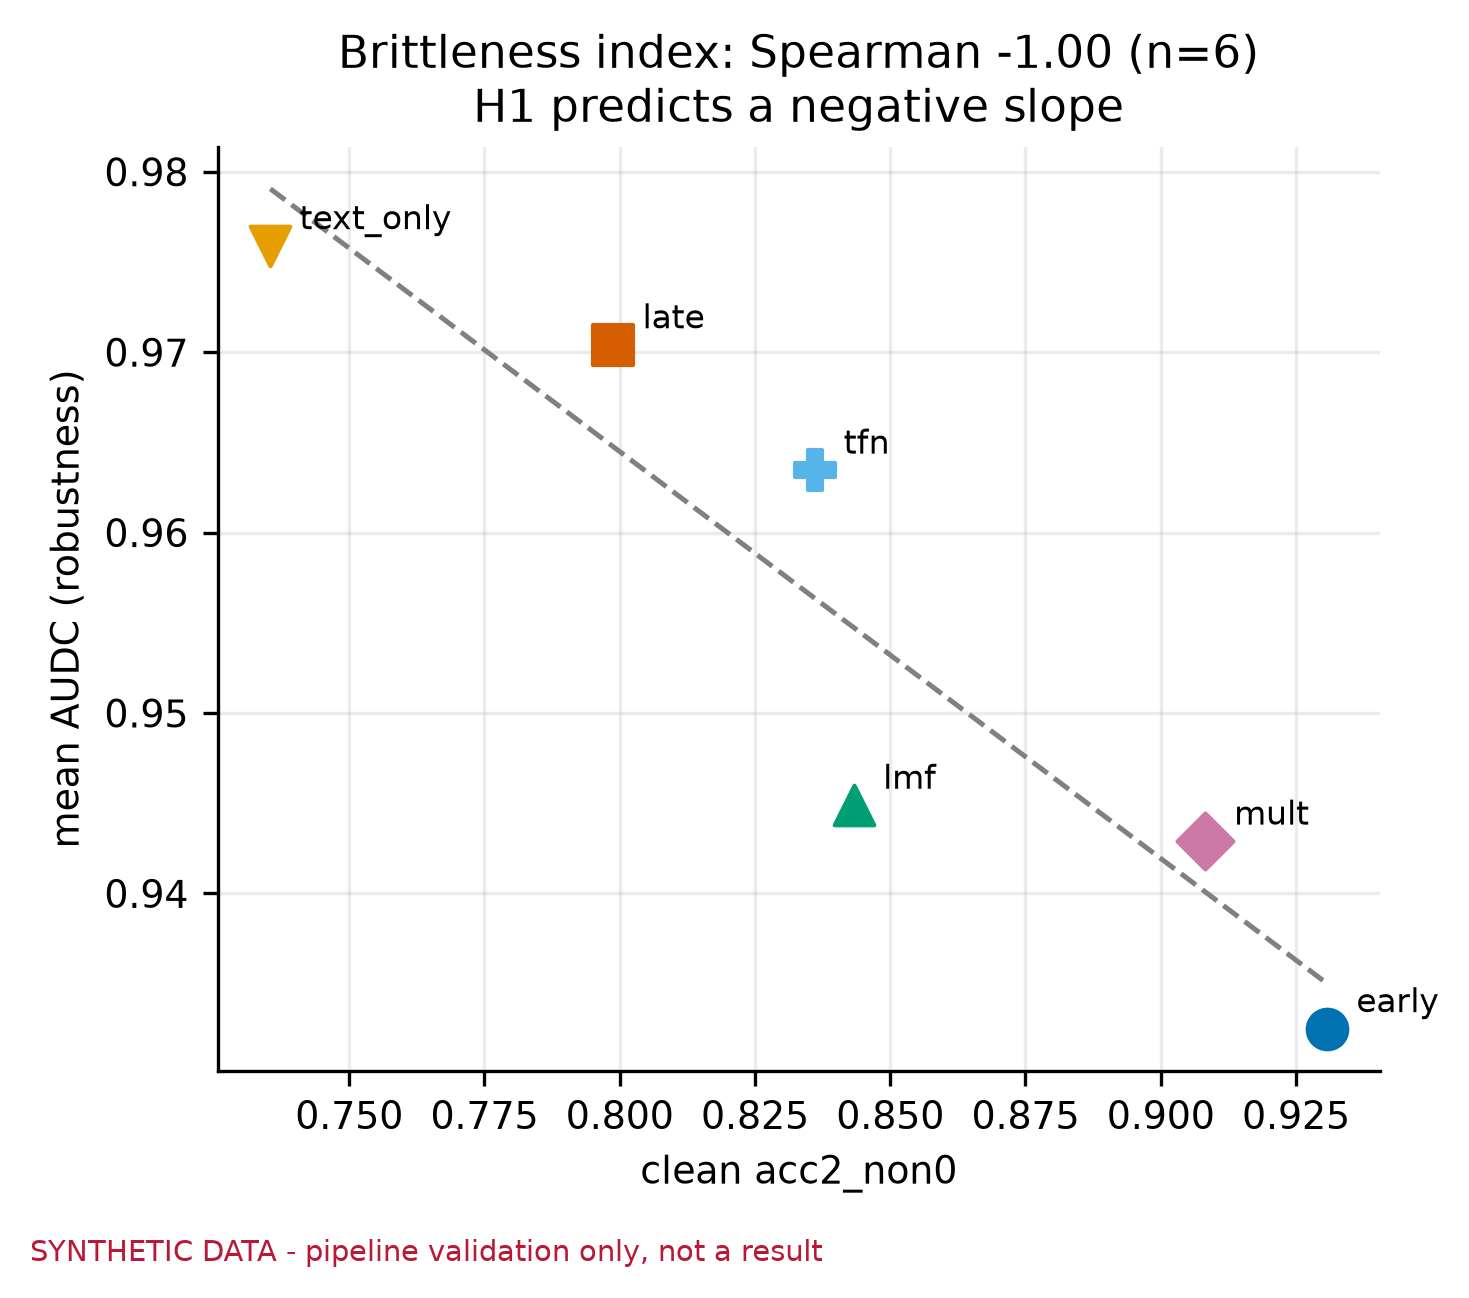
\includegraphics[width=0.72\textwidth]{figures/fig3_brittleness.png}
  \caption{Clean performance against mean AUDC across architectures. H1 predicts a
           negative slope.}
  \label{fig:brittleness}
\end{figure}

\begin{figure}[t]
  \centering
  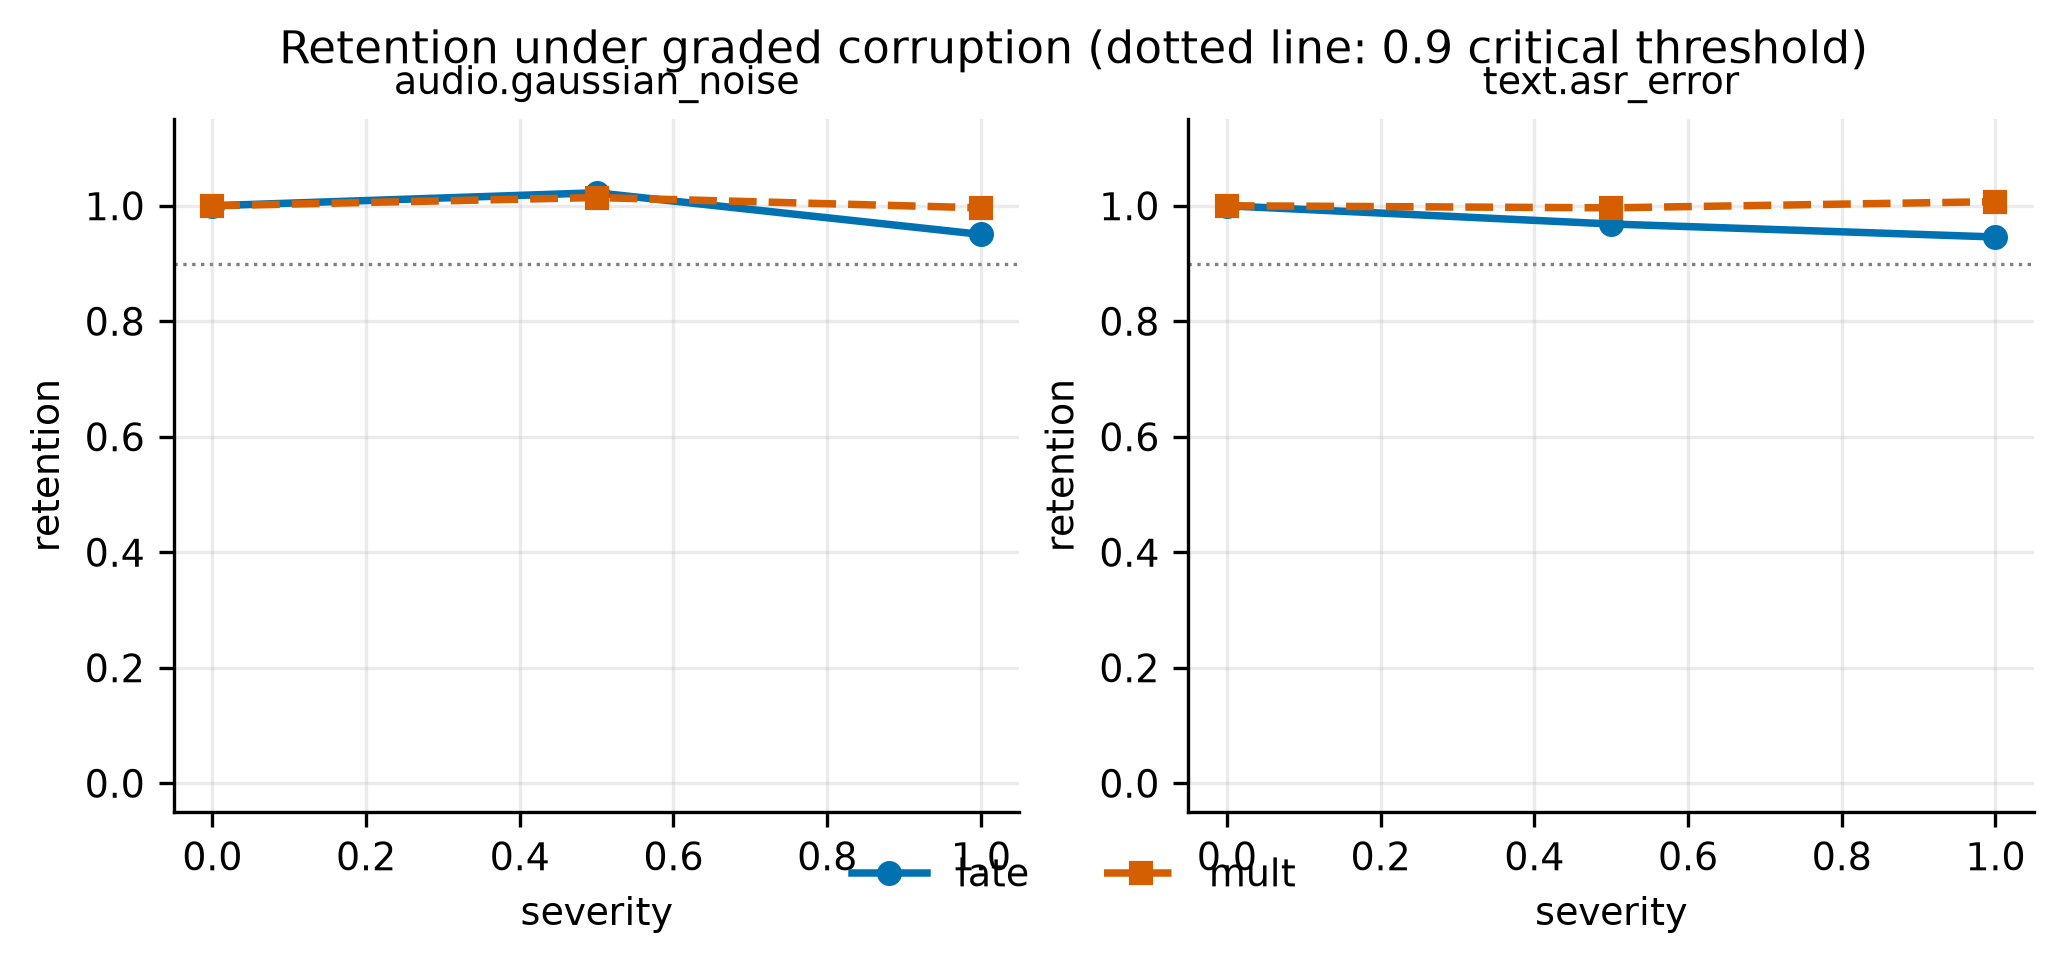
\includegraphics[width=\textwidth]{figures/fig1_degradation_curves.png}
  \caption{Retention under graded corruption, faceted by corruption family. Bands are
           $\pm 1$ std over five seeds; the dotted line marks the 0.9 critical threshold.}
  \label{fig:curves}
\end{figure}

\subsection{Q2: reliance asymmetry}
\begin{figure}[t]
  \centering
  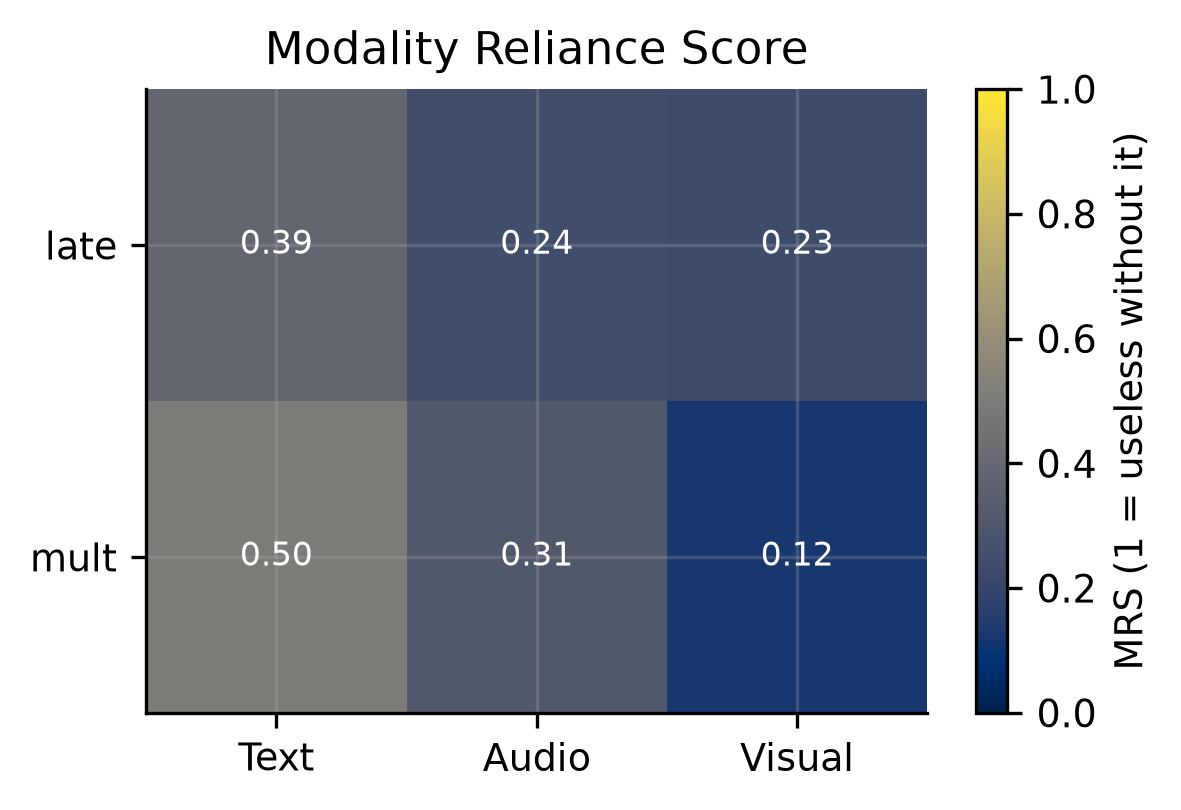
\includegraphics[width=0.6\textwidth]{figures/fig2_modality_reliance.png}
  \caption{Modality Reliance Score by architecture.}
  \label{fig:reliance}
\end{figure}

\subsection{Q3: does modality dropout buy robustness, and at what price?}
\begin{figure}[t]
  \centering
  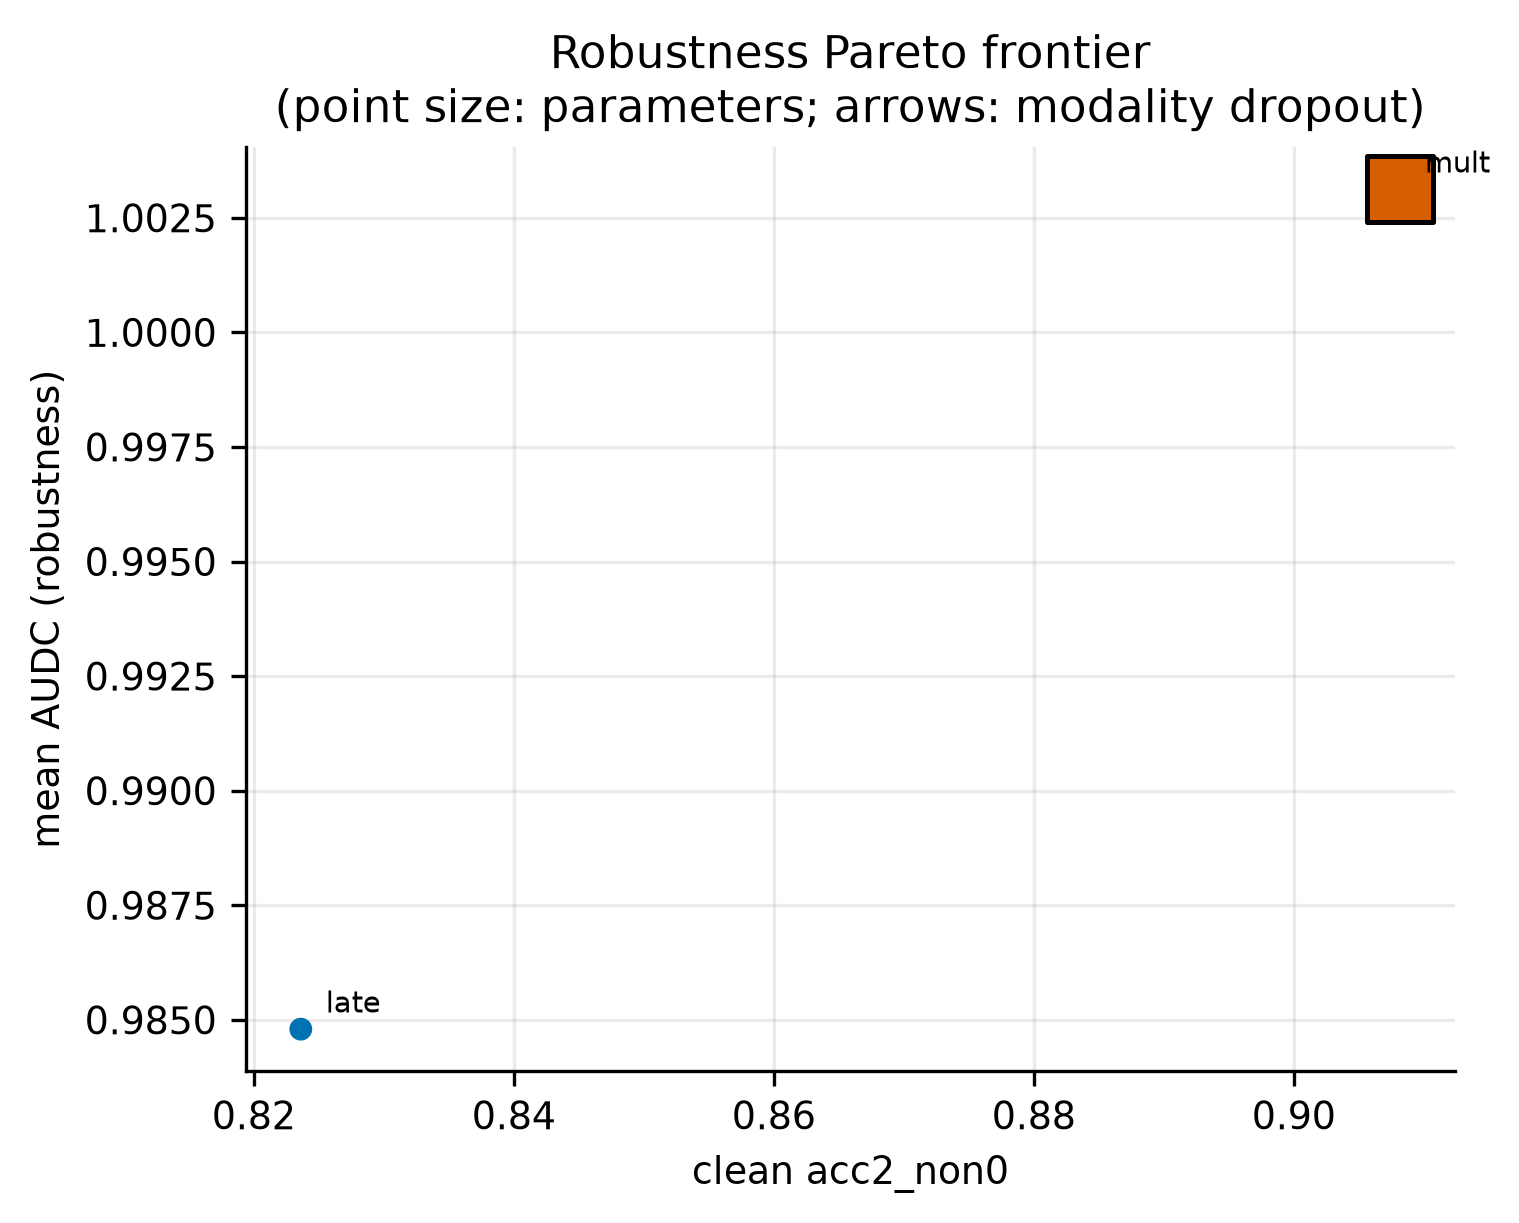
\includegraphics[width=0.7\textwidth]{figures/fig4_pareto.png}
  \caption{Clean performance against robustness. Arrows link each modality-dropout
           variant to its untrained-for-robustness control.}
  \label{fig:pareto}
\end{figure}

\subsection{Q4: graded versus binary corruption}
% Does degraded input behave like partial absence, or differently?

\section{Discussion}
% If H1 is disconfirmed, say so plainly and explain why. A clean disconfirmation is a
% more interesting result than a mild confirmation, and panels select for that honesty.

\section{Limitations}
% Corruption is applied in feature space, not to raw media — deliberate (three orders of
% magnitude cheaper, and every architecture provably sees the same tensor), but it means
% the ASR channel is simulated rather than measured from a real recogniser.
% Precomputed GloVe/COVAREP/Facet features rather than end-to-end encoders.
% Two datasets, both English, both from a narrow set of recording conditions.

\section{Conclusion}

\bibliographystyle{plainnat}
\bibliography{references}

\end{document}
